\documentclass[12pt]{article}

\usepackage[a4paper, left=1.2in, right=1.2in]{geometry}
\usepackage{setspace}
\usepackage[utf8]{inputenc}
\usepackage[italian]{babel}
\usepackage[OT1]{fontenc}
\usepackage{graphicx}
\usepackage{subcaption}
\usepackage{float}
\usepackage{fancyhdr}
\usepackage{xcolor}
\usepackage{mathtools}
\usepackage{amsmath}
\usepackage{amssymb}
\usepackage{tikz}
\usepackage{imakeidx}
\usepackage{textcomp}
\usepackage{pifont}
\usepackage{polynom}
\usepackage{algorithm}
\usepackage{algpseudocode}
\usepackage{mathtools}
\usepackage{cancel}
\usepackage{pgfplots}
\usepackage{caption}
\usepackage{tabularx}
\usepackage{comment}
\usepackage{float}
\usepackage{bm}
\usepackage{multirow}
\usepackage{listings}
\usepackage{longtable}
\usepackage[colorlinks=true,linkcolor=black,anchorcolor=black,citecolor=black,filecolor=black,menucolor=black,runcolor=black,urlcolor=black,backref=page]{hyperref}
\begin{document}

% colors
\definecolor{drawgray}{HTML}{666666}
\definecolor{drawgray_l}{HTML}{F5F5F5}
\definecolor{drawblue}{HTML}{6C8EBF}
\definecolor{drawblue_l}{HTML}{DAE8FC}
\definecolor{drawgreen}{HTML}{82B366}
\definecolor{drawgreen_l}{HTML}{D5E8D4}
\definecolor{draworange}{HTML}{D79B00}
\definecolor{draworange_l}{HTML}{FFE6CC}
\definecolor{drawyellow}{HTML}{D6B656}
\definecolor{drawyellow_l}{HTML}{FFF2CC}
\definecolor{drawred}{HTML}{B85450}
\definecolor{drawred_l}{HTML}{EA6B66}
\definecolor{drawviolet}{HTML}{9673A6}
\definecolor{drawviolet_l}{HTML}{E1D5E7}
\definecolor{drawblackish}{HTML}{422222}

\definecolor{deepblue}{rgb}{0,0,0.5}
\definecolor{deepgreen}{rgb}{0,0.5,0}


\lstset{ 
  language=Python,
  framesep=1pt,
  xleftmargin=0pt,
  framexleftmargin=0pt,
  frame=tb,
  framerule=1pt,
  breaklines=true,
  keywordstyle=\color{blue}\bfseries,
  showstringspaces=false
}

\lstset{ 
  language=SQL,
  morekeywords={AFTER, INSTEAD, OF, REFERENCING, FOR, EACH, ROW, DECLARE, IF, TYPE, NEW, RETURNS, SELF, BEGIN, END, CONSTRUCTOR, UNDER, CONSTRUCTOR, STATIC, INSTANCE, RETURN, OVERRIDING, FINAL, NOT, INSTANTIABLE, UNNEST, MULTISET, ARRAY, COLLECT, METHOD, REF, MEMBER, FUNCTION, PROCEDURE, PRAGMA, RESTRICT_REFERENCES, WNDS, RNDS, TABLE, WITH, ASSIGNMENT, OPTIONS, SCOPE, NESTED, STORE, DEREF, VARRAY, OBJECT, DBMS_OUTPUT, PUT_LINE, INSERTING, UPDATING, THEN, FOR, LOOP, EXTEND, REF, TRUNC, DBMS_RANDOM, TO_CHAR, TO_DATE, PROCEDURE, REPLACE, BEFORE, COMPOUND, OLD, RAISE_APPLICATION_ERROR, SYSDATE, STATEMENT, IS, ROUND, NVL, ELSIF, DUAL, RAWTOHEX, GUID, SYS},
  framesep=1pt,
  xleftmargin=0pt,
  framexleftmargin=0pt,
  frame=tb,
  framerule=1pt,
  breaklines=true,
  commentstyle=\color{deepgreen},
  keywordstyle=\color{deepblue},
  showstringspaces=false,
  mathescape
}
\renewcommand{\tablename}{Table}
\renewcommand{\figurename}{Figure}
\begin{titlepage}
    \begin{center}
        
\includegraphics[scale=0.5]{images/uniba-logo.png}\\
        \vspace{0.5cm}
        % Dipartimento
        {\large COMPUTER SCIENCE DEPARTMENT}\\
        \vspace{0.5cm}
        % Corso di laurea
        {\large Computer Science - Curriculum Artificial Intelligence}\\
        \hrulefill \\
        \vspace{0.5cm}
        {\large Project Assignment}\\
        \vspace{0.5cm}
        % Materia
        {\large Database Systems}\\
        \vspace{0.5cm}
        % Titolo
        {\LARGE \textbf{Database Design and Implementation}}\\
        %% \textbf{Titolo della Tesi} 
        \vspace{0.5cm}

        \vfill
        \centering
        \begin{tabularx}{\textwidth}{@{}Xr@{}}
          % Relatore
          {\large Student:} &
          {\large \textit{Fontana Emanuele}} \\ 
        \end{tabularx}
        \textcolor{white}{.} \\ 
        \vspace{0.5cm}
        \hrulefill \\
        % Anno accademico in cui si è iscritti
        {\large Academic Year 2024/2025}
    \end{center}
\end{titlepage}
\newpage
\tableofcontents
\newpage
\section{Conceptual Design}
\subsection{Requirements}
The requirements for the database are the following:
\begin{table}[H]
    \renewcommand{\arraystretch}{1.3} % Adjust row height
    \begin{tabularx}{\textwidth}{|X|}
    \hline
    \textbf{"GreenWorld Energy"} \\ \hline
    The company "GreenWorld Energy" operates decentralized renewable energy production facilities distributed 
across regions. Each facility is characterized by a name, location, type of energy produced (e.g., solar, wind, 
hydro), and maximum energy output capacity. The company also manages contracts with customers for energy 
supply, categorized as residential or commercial, and offers flexible pricing models based on consumption. 
Each customer has one or more accounts, each identified by a unique code. Every energy contract is linked to a 
single customer account and includes details such as start date, duration, energy plan, and cost. Facilities are 
overseen by management teams, each identified by a unique code, team name, and the number of projects managed. 
Teams are evaluated based on performance metrics such as energy efficiency, uptime, and customer satisfaction. 
Each team is represented by the main responsible employee and other employees identified by fiscal code, name, 
surname, date of birth and date of hiring. Additionally, the company supports a feedback system allowing 
customers to submit ratings and comments regarding service quality. Customers are classified into residential and 
commercial types, each identified by a unique alphanumeric code, with associated contact details and energy 
consumption history. \\ \hline
    \end{tabularx}
    \caption{Requirements}
    \end{table}


\subsection{Analysis}

\subsubsection{Glossary of Terms}
\begin{table}[H]
    \renewcommand{\arraystretch}{1.3} % Adjust row height
    \begin{tabularx}{\textwidth}{|X|X|X|X|}
    \hline
    \textbf{Term}& \textbf{Description}  & \textbf{Connections}    & \textbf{Synonyms}     \\ \hline
    Region      & Area where the facilities are located. & Facility     & Location \\ \hline
    Facility     & Energy production facility. It emits energy for customers      & Contract,Teams,Region         &\\ \hline
    Contract     & Energy supply contract. It describes the energy plan. It can be residential or commercial & Account, Facility     & Projects        \\ \hline
    Customer     & Customer of GreenWorld Energy. It can be residential or commercial       & Account    &        \\ \hline
    Account      & Customer account. It associated with only one account and one contract & Contract, Customer, Feedback     &        \\ \hline
    Feedback     & Customer feedback. Used to give a score to each team       & Account,Team     &         Ratings, customer satisfaction \\\hline
    Team        & Groups of employees that oversees a facility. Each team has a manager       & Facility, Employee, Feedback     &        \\ \hline
    Employee     & Employee of a GreenWorld Energy's team.      & Team     &        \\ \hline
    \end{tabularx}
    \caption{Glossary of Terms}
    \end{table}
\newpage
\subsubsection{Level of Abstraction}
By considering the synonyms of the terms, we can identify the level of abstraction of the terms. The terms can be classified as follows:
\begin{itemize}
    \item \textbf{Region} as Location
    \item \textbf{Facility} as Facility
    \item \textbf{Contract} as Contract
    \item \textbf{Customer} as Customer
    \item \textbf{Account} as Account
    \item \textbf{Feedback} as Feedback
    \item \textbf{Team} as Team
    \item \textbf{Employee} as Employee
\end{itemize}

\subsubsection{Reorganization of Concepts}
The concepts can be reorganized as follows:
\begin{table}[H]
    \renewcommand{\arraystretch}{1.3} % Adjust row height
    \begin{tabularx}{\textwidth}{|X|}
    \hline  \textbf{Facility}    \\ \hline
    Each facility is characterized by a name, location, type of energy produced (e.g., solar, wind, hydro), and maximum energy output capacity. The company also manages contracts with customers for energy supply, categorized as residential or commercial, and offers flexible pricing models based on consumption. Facilities are overseen by management teams \\ \hline
    \end{tabularx}
    \caption{Facility's Concepts}
    \end{table}

\begin{table}[H]
    \renewcommand{\arraystretch}{1.3} % Adjust row height
    \begin{tabularx}{\textwidth}{|X|}
    \hline  \textbf{Contract}    \\ \hline
    The company also manages contracts with customers for energy supply, categorized as residential or commercial, and offers flexible pricing models based on consumption.
    Every enegry contract is linked to a single customer account and includes details such as start date, duration, energy plan, and cost. \\ \hline
    \end{tabularx}
    \caption{Contract's Concepts}
    \end{table}

\begin{table}[H]
    \renewcommand{\arraystretch}{1.3} % Adjust row height
    \begin{tabularx}{\textwidth}{|X|}
    \hline  \textbf{Customer}    \\ \hline
    Each customer has one or more accounts, each identified by a unique code. Customers are classified into residential and commercial types, each identified by a unique alphanumeric code, with associated contact details and energy consumption history. Additionally, the company supports a feedback system allowing customers to submit ratings and comments regarding service quality. \\ \hline
    \end{tabularx}
    \caption{Customer's Concepts}
    \end{table}

\begin{table}[H]
    \renewcommand{\arraystretch}{1.3} % Adjust row height
    \begin{tabularx}{\textwidth}{|X|}
    \hline   \textbf{Account}    \\ \hline
    Each customer has one or more accounts, each identified by a unique code. Every energy contract is linked to a single customer account and includes details such as start date, duration, energy plan, and cost. \\ \hline
    \end{tabularx}
    \caption{Account's Concepts}
    \end{table}

\begin{table}[H]
    \renewcommand{\arraystretch}{1.3} % Adjust row height
    \begin{tabularx}{\textwidth}{|X|}
    \hline  \textbf{Feedback}    \\ \hline
    The company supports a feedback system allowing customers to submit ratings and comments regarding service quality. \\ \hline
    \end{tabularx}
    \caption{Feedback's Concepts}
    \end{table}

\begin{table}[H]
    \renewcommand{\arraystretch}{1.3} % Adjust row height
    \begin{tabularx}{\textwidth}{|X|}
    \hline  \textbf{Team}    \\ \hline
    Facilities are overseen by management teams, each identified by a unique code, team name, and the number of projects managed. Teams are evaluated based on performance metrics such as energy efficiency, uptime, and customer satisfaction. Each team is represented by the main responsible employee \\ \hline
    \end{tabularx}
    \caption{Team's Concepts}
    \end{table}

\begin{table}[H]
    \renewcommand{\arraystretch}{1.3} % Adjust row height
    \begin{tabularx}{\textwidth}{|X|}
    \hline  \textbf{Employee}    \\ \hline
    Each team is represented by the main responsible employee and other employees identified by fiscal code, name, surname, date of birth and date of hiring. \\ \hline
    \end{tabularx}
    \caption{Employee's Concepts}
    \end{table}

\subsubsection{Entity-Relationship Diagram}

\paragraph{SKELETON SCHEMA} \leavevmode \newline
\begin{figure}[H]
    \centering
    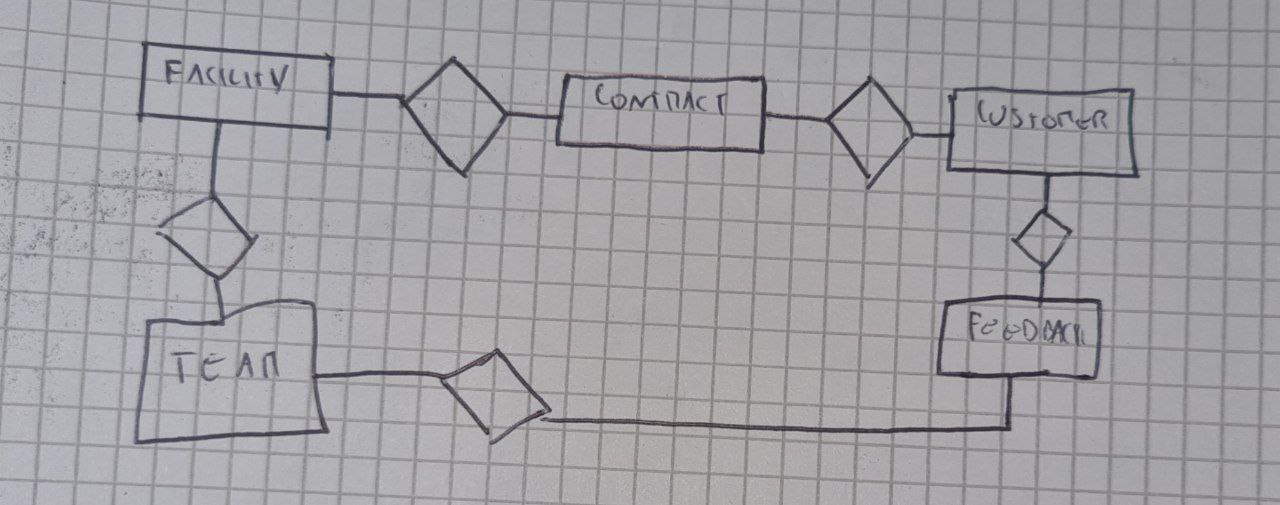
\includegraphics[width=\textwidth]{images/SkeletonSchema.png}
    \caption{Skeleton Schema}
\end{figure}

\noindent This schema represents the main entities and their relationships. The entities are the following:
\begin{itemize}
    \item \textbf{Facility}
    \item \textbf{Contract}
    \item \textbf{Customer}
    \item \textbf{Feedback}
    \item \textbf{Team}
\end{itemize}
The purpose of this schema is to have a general idea of the entities and their relationships. The attributes of the entities and the cardinality of the relationships are not included in this schema. Also, some entities are not included in this schema, such as Account and Employee. These entities will be included in the final schema with all the other details.

\paragraph{FINAL SCHEMA} \leavevmode \newline

\begin{figure}[H]
    \centering
    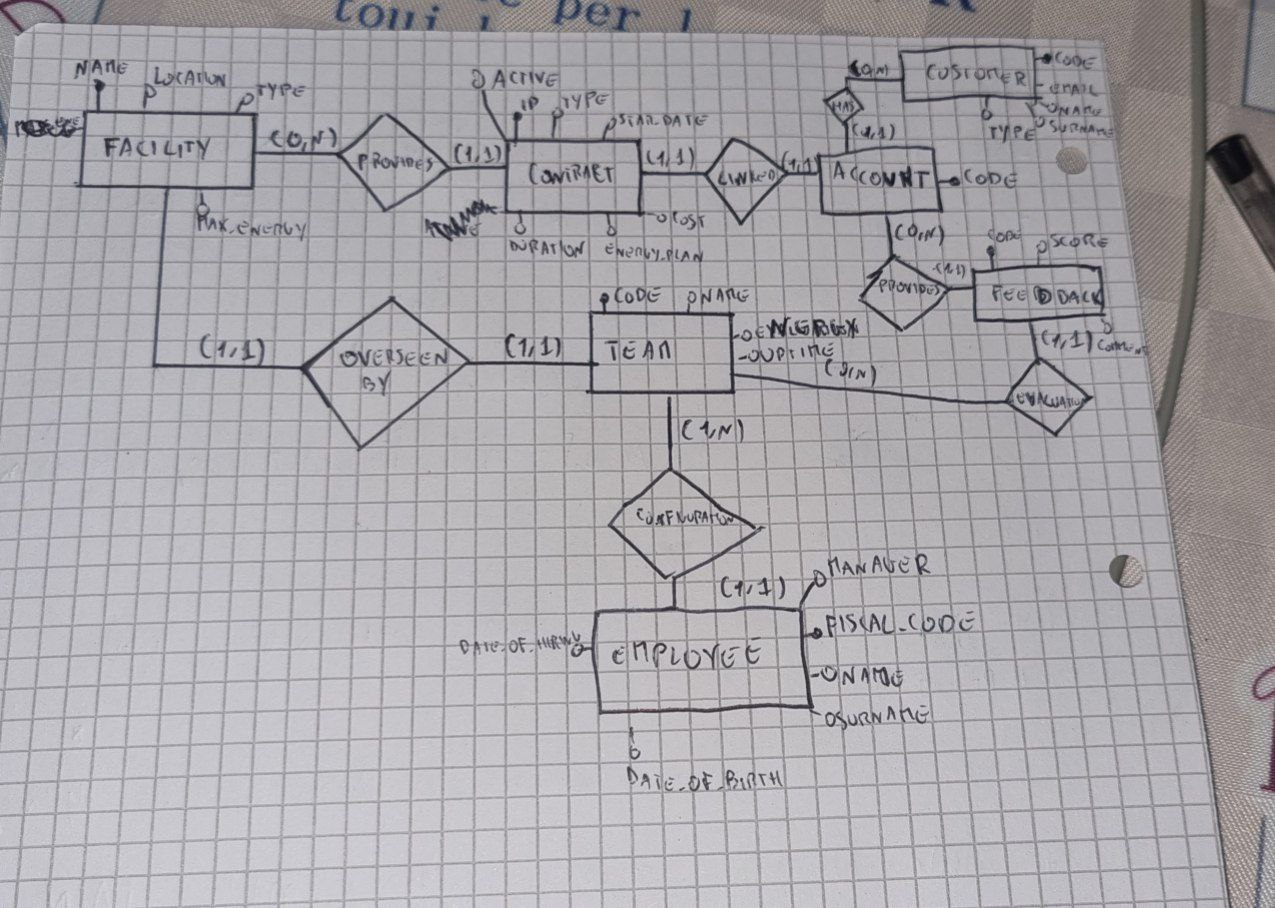
\includegraphics[width=\textwidth]{images/ER.png}
    \caption{Final Schema}
\end{figure}


\subsubsection{Business Rules}
The business rules are the following:
\begin{itemize}
    \item A customer can't be a minor
    \item An employee can't be a minor
    \item Each team has got only one main responsible employee
    \item The sum of energy plan of all contracts related to a facility can't exceed the maximum energy output capacity of the facility
    \item If an account needs to activate a new contract with the same facility, the old contract must deactivated before the new one is activated
    \item A customer of a specific type can't have a contract of the other type
    \item The score of a feedback can be between 0 and 5
    \item Uptime is the number of hours the facility is active in a day. Between 6 and 8
    \item Energy efficiency is the percentage of energy produced compared to the maximum energy output capacity of the facility. Between 0 and 100
\end{itemize}




\newpage
\section{Logical Design}

\subsection{Volume Table}
Lets consider the volumes for a year

\begin{table}[H]
    \scriptsize
    \renewcommand{\arraystretch}{1.3} % Adjust row height
    \begin{tabularx}{\textwidth}{|X|X|X|X|}
    \hline
    \textbf{Concept}& \textbf{Type}  & \textbf{Volume}    & \textbf{Description}     \\ \hline
    Facility & E & 100 & Number of facilities (Given) \\ \hline
    Contract & E & 900.000 & Number of contracts. 100 facilities * 500 contracts per facility * 12 months * 1.5 contracts per account \\ \hline
    Customer & E & 300.000 & Number of customers.(ASSUMPTION) \\ \hline
    Account & E & 600.000 & Number of accounts. 300.000 customers * 2 accounts per customer on average\\ \hline
    Team & E & 50 & Number of teams. (ASSUMPTION) \\ \hline
    Employee & E & 250 & Number of employees. 5 employees per team * 50 teams (ASSUMPTION) \\ \hline
    Feedback & E & 600.000 & Number of feedbacks.\\ \hline
    Provides & R & 900.000 & Each contract is provided by a single facility \\ \hline
    Linked & R & 900.000 & On average each account has 1.5 contracts \\ \hline
    Has & R & 600.000 & Each customer 2 accounts on average \\ \hline
    OverseenBy & R & 100 & Each facility is overseen by a single team. Each team oversees 2 facilities, on average \\ \hline
    Configuration & R & 500 & Each team constists of 5 employees on average \\ \hline
    Gives & R & 500.000 & Each feedback is given by a single account.Not all accounts give feedback  \\ \hline
    Evaluation & R & 500.000 & Each feedback is linked to a single team\\ \hline
    \end{tabularx}
    \caption{Volume Table}
\end{table}

\subsection{Access Table}

\textbf{Operation1:} Register a new customer (50 times per day)\\
\begin{table}[H]
    \renewcommand{\arraystretch}{1.3} % Adjust row height
    \begin{tabularx}{\textwidth}{|X|X|X|X|}
    \hline
    \textbf{Concept}& \textbf{Type}  & \textbf{Access}    & \textbf{Type}     \\ \hline
    Customer & E & 1 & W \\ \hline
    \end{tabularx}
    \caption{Access Table for Operation1}
\end{table}
\noindent Total Cost: 2 * 50 = 100 per day
\newline
\textbf{Operation2:} Register a new energy contract (50 times per day)\\
\begin{table}[H]
    \renewcommand{\arraystretch}{1.3} % Adjust row height
    \begin{tabularx}{\textwidth}{|X|X|X|X|}
    \hline
    \textbf{Concept}& \textbf{Type}  & \textbf{Access}    & \textbf{Type}     \\ \hline
    Contract & E & 1 & W \\ \hline
    Provides & R & 1 & W \\ \hline
    Facility & E & 1 & R \\ \hline
    Linked & R & 1 & W \\ \hline
    Account & E & 1 & R \\ \hline
    Facility & E & 1 & W \\ \hline
    Provides & R & 9000 & R \\ \hline
    Contract & E & 9000 & R \\ \hline
    \end{tabularx}
    \caption{Access Table for Operation2}
\end{table}
\noindent Total Cost: (2+2+1+2+1+2+9000+9000)*200=3.602.000 per day

\noindent Every time we need to update the efficiency score of the facility related to the contracts.
\newline
\noindent \textbf{Operation3:} Assign a facility to a management team (50 times per day)\\
\begin{table}[H]
    \renewcommand{\arraystretch}{1.3} % Adjust row height
    \begin{tabularx}{\textwidth}{|X|X|X|X|}
    \hline
    \textbf{Concept}& \textbf{Type}  & \textbf{Access}    & \textbf{Type}     \\ \hline
    Team & E & 1 & R \\ \hline
    OverseenBy & R & 1 & W \\ \hline
    Facility & E & 1 & R \\ \hline
    \end{tabularx}
    \caption{Access Table for Operation3}
\end{table}
\noindent Total Cost: (1+2+1)*50=200 per day
\newline
\noindent \textbf{Operation4:} View the total energy output of a specific facility managed by the eldest employee (1 per month = 0.03 per day)\\
\begin{table}[H]
    \renewcommand{\arraystretch}{1.3} % Adjust row height
    \begin{tabularx}{\textwidth}{|X|X|X|X|}
    \hline
    \textbf{Concept}& \textbf{Type}  & \textbf{Access}    & \textbf{Type}     \\ \hline
    Employee & E & 250 & R \\ \hline
    Configuration & R & 1 & R \\ \hline
    Team & E & 1 & R \\ \hline
    OverseenBy & R & 2 & R \\ \hline
    Facility & E & 2 & R \\ \hline
    Provides & R & 9000 & R \\ \hline
    Contract & E & 9000 & R \\ \hline
    \end{tabularx}
    \caption{Access Table for Operation4}
\end{table}
\noindent Total Cost: (250+1+1+1+2+9000+9000)*0.03=547.65 per day
\newline
\noindent Each team oversees, on average, twow facilities. We need to choose only one of them, which provides on average 9000 contracts.
In this case we don't have sumEnergyOutput in the schema as attribute of the facility, so we need to compute it every time. If we introduce it, the cost will be
\begin{table}[H]
    \renewcommand{\arraystretch}{1.3} % Adjust row height
    \begin{tabularx}{\textwidth}{|X|X|X|X|}
    \hline
    \textbf{Concept}& \textbf{Type}  & \textbf{Access}    & \textbf{Type}     \\ \hline
    Employee & E & 250 & R \\ \hline
    Configuration & R & 1 & R \\ \hline
    Team & E & 1 & R \\ \hline
    OverseenBy & R & 2 & R \\ \hline
    Facility & E & 2 & R \\ \hline
    \end{tabularx}
    \caption{Access Table for Operation4 with redundancy}
\end{table}
\noindent Total Cost: (250+1+1+2+2)*0.03=7.68 per day
\newline
\noindent But in this case we need to update it every time we add a new contract, so the total cost of \textbf{Operation2} will be:

\begin{table}[H]
    \renewcommand{\arraystretch}{1.3} % Adjust row height
    \begin{tabularx}{\textwidth}{|X|X|X|X|}
    \hline
    \textbf{Concept}& \textbf{Type}  & \textbf{Access}    & \textbf{Type}     \\ \hline
    Contract & E & 1 & W \\ \hline
    Provides & R & 1 & W \\ \hline
    Facility & E & 1 & R \\ \hline
    Facility & E & 1 & W \\ \hline
    Linked & R & 1 & W \\ \hline
    Account & E & 1 & R \\ \hline
    Facility & E & 1 & W \\ \hline
    Provides & R & 9000 & R \\ \hline
    Contract & E & 9000 & R \\ \hline
    \end{tabularx}
    \caption{Access Table for Operation2 with redundancy}
\end{table}
\noindent Total Cost: (2+2+1+2+2+1+2+9000+9000)*200=3.602.400 per day
\newline
\noindent So the total cost without redundancy is 3.602.000 +547.65 = 3.602.547.65, while the total cost with redundancy is 3.602.400 + 7.68 = 3.602.407.68 per day. So we should keep the redundancy in this case. 
\newline
\noindent \textbf{Operation5:} Print a ranked list of facilities based on their efficiency scores (10 per day)
\begin{table}[H]
    \renewcommand{\arraystretch}{1.3} % Adjust row height
    \begin{tabularx}{\textwidth}{|X|X|X|X|}
    \hline
    \textbf{Concept}& \textbf{Type}  & \textbf{Access}    & \textbf{Type}     \\ \hline
    Facility & E & 100 & R \\ \hline
    \end{tabularx}
    \caption{Access Table for Operation5}
\end{table}
\noindent Total Cost: 100*10 = 1000 per day

\noindent We can try to remove the redundancy of the efficiencyScore in facilities
\begin{table}[H]
\renewcommand{\arraystretch}{1.3} % Adjust row height
\begin{tabularx}{\textwidth}{|X|X|X|X|}
\hline
\textbf{Concept}& \textbf{Type}  & \textbf{Access}    & \textbf{Type}     \\ \hline
Facility & E & 100 & R \\ \hline
Provides & R & 900.000 & R \\ \hline
Contract & E & 900.000 & R \\ \hline
\end{tabularx}
\caption{Access Table for Operation5 without redundancy}
\end{table}
\noindent Total Cost: (100+900.000+900.000)*10 = 18.001.000 per day 
\begin{table}[H]
    \renewcommand{\arraystretch}{1.3} % Adjust row height
    \begin{tabularx}{\textwidth}{|X|X|X|X|}
    \hline
    \textbf{Concept}& \textbf{Type}  & \textbf{Access}    & \textbf{Type}     \\ \hline
    Contract & E & 1 & W \\ \hline
    Provides & R & 1 & W \\ \hline
    Facility & E & 1 & R \\ \hline
    Linked & R & 1 & W \\ \hline
    Account & E & 1 & R \\ \hline
    \end{tabularx}
    \caption{Access Table for Operation2 without redundancy}
\end{table}
\noindent Total Cost: (2+2+1+2+1)*200=1.600 per day
\newline
\noindent Now we don't need to update the the efficiency score everytime we register a new contract.

\noindent So the total cost without redundancy is 18.002.600, while the total cost with redundancy is 2.402.000 + 1000 = 2.403.000 per day.

\noindent We shouuld keep the redundancy in this case.

\subsubsection{Redundancies and Generalization}
\begin{itemize}
    \item \textbf{Redundancies:} The number of facilities managed by a team is not stored in the schema, as it can be calculated by counting the number of facilities managed by the team. The score of the team can be derived by the following formula: $score = \frac{energy\_efficiency + uptime + AVG(customer\_score)}{3}$ and is not stored in the schema to avoid redundancy. Due to the previous analysis, the redundancy of the efficiency score and sumEngergyOutput in the facility are kept in the schema
    \item \textbf{Generalization:} The schema doesn't contain any generalization since there aren't different operations for them. There is a \textbf{type} attribute in the \textbf{Customer} and \textbf{Contract} entities so that the business rule related to the type of contract can be enforced.
\end{itemize}


\subsection{UML Schema}

\begin{figure}[H]
    \centering
    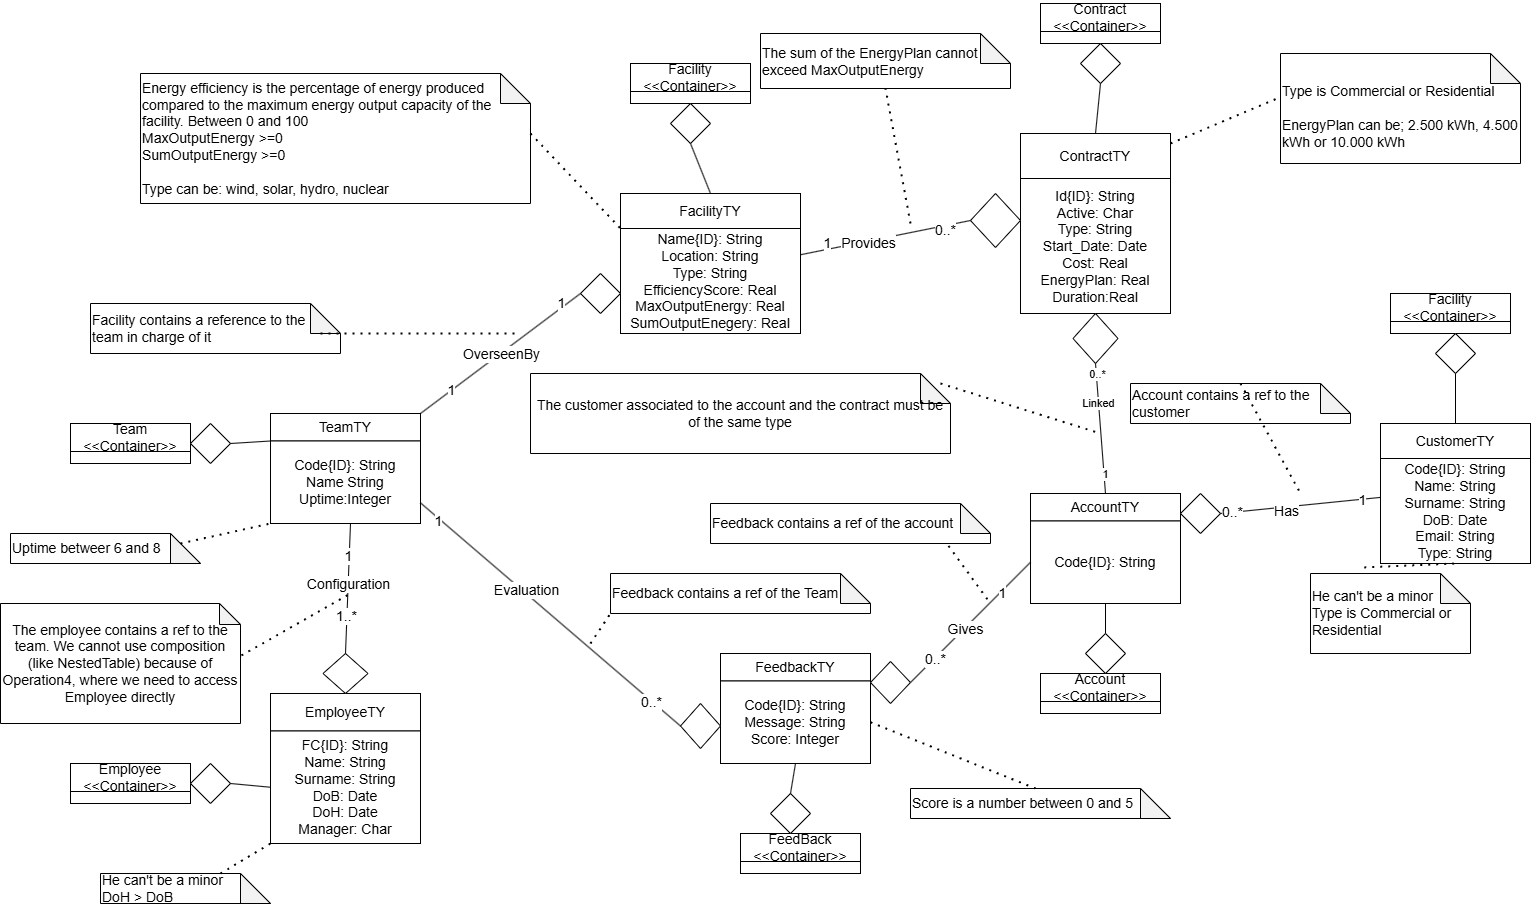
\includegraphics[width=\textwidth]{images/UML.png}
    \caption{UML Schema}
\end{figure}

\newpage
\section{Implementation}
\subsection{Types Definition}

\begin{lstlisting}
    CREATE OR REPLACE TYPE TeamTY AS OBJECT (
        Code VARCHAR2(20),
        Name VARCHAR2(50),
        Uptime INTEGER
    )
\end{lstlisting}

\begin{lstlisting}
    CREATE OR REPLACE TYPE FacilityTY AS OBJECT (
        Name VARCHAR2(50),
        Location VARCHAR2(100),
        Type VARCHAR2(20),
        EfficiencyScore NUMBER,
        MaxOutputEnergy NUMBER,
        SumOutputEnergy NUMBER,
        Team REF TeamTY)
\end{lstlisting}

\begin{lstlisting}
    CREATE OR REPLACE TYPE EmployeeTY AS OBJECT (
        FC VARCHAR2(20),
        Name VARCHAR2(50),
        Surname VARCHAR2(50),
        DoB DATE,
        DoH DATE,
        Manager CHAR(1),
        Team REF TeamTY
    )
\end{lstlisting}


\begin{lstlisting}
    CREATE OR REPLACE TYPE CustomerTY AS OBJECT (
        Code VARCHAR2(20),
        Name VARCHAR2(50),
        Surname VARCHAR2(50),
        Email VARCHAR2(100),
        Type VARCHAR2(20),
        DoB DATE
    )
\end{lstlisting}


\begin{lstlisting}
CREATE OR REPLACE TYPE AccountTY AS OBJECT (
    Code VARCHAR2(20),
    Customer REF CustomerTY
    )
\end{lstlisting}



\begin{lstlisting}
CREATE OR REPLACE TYPE ContractTY AS OBJECT (
        ID VARCHAR2(20),
        Active CHAR(1),
        Type VARCHAR2(20),
        Start_Date DATE,
        Cost NUMBER,
        EnergyPlan NUMBER,
        Duration NUMBER,
        Account REF AccountTY,
        Facility REF FacilityTY
    )
\end{lstlisting}


\begin{lstlisting}
    CREATE OR REPLACE TYPE FeedbackTY AS OBJECT (
        Code VARCHAR2(20),
        Message VARCHAR2(200),
        Score INTEGER,
        Account REF AccountTY ,
        Team REF TeamTY
    )
\end{lstlisting}

\subsection{Tables Definition}

\begin{lstlisting}
    CREATE TABLE Team OF TeamTY (
        Code PRIMARY KEY,
        CONSTRAINT chk_uptime CHECK (Uptime BETWEEN 6 AND 8),
        Name NOT NULL,
        Uptime NOT NULL
    )
\end{lstlisting}

We can see that simple constraints are handled with \textbf{check}

\begin{lstlisting}
    CREATE TABLE Facility OF FacilityTY (
        Name PRIMARY KEY,
        CONSTRAINT chk_facility_type CHECK (Type IN (''wind'', ''solar'', ''hydro'', ''nuclear'')),
        CONSTRAINT chk_max_output_energy CHECK (MaxOutputEnergy >= 0),
        CONSTRAINT chk_sum_output_energy CHECK (SumOutputEnergy >= 0),
        Location NOT NULL,
        Type NOT NULL,
        MaxOutputEnergy NOT NULL,
        EfficiencyScore NOT NULL,
        Team REFERENCES Team ON DELETE SET NULL
    )
\end{lstlisting}


\begin{lstlisting}
    CREATE TABLE Employee OF EmployeeTY (
        FC PRIMARY KEY,
        CONSTRAINT chk_manager CHECK (Manager IN (''Y'', ''N'')),
        Name NOT NULL,
        Surname NOT NULL,
        DoB NOT NULL,
        DoH NOT NULL,
        Manager NOT NULL,
        CONSTRAINT chk_doh_after_dob CHECK (DoH > DoB),
        Team REFERENCES Team ON DELETE SET NULL
    )
\end{lstlisting}


\begin{lstlisting}
    CREATE TABLE Customer OF CustomerTY (
        Code PRIMARY KEY,
        CONSTRAINT chk_customer_type CHECK (Type IN (''Commercial'', ''Residential'')),
        Name NOT NULL,
        Surname NOT NULL,
        Email NOT NULL,
        Type NOT NULL,
        DoB NOT NULL
    )
\end{lstlisting}



\begin{lstlisting}
    CREATE TABLE Account OF AccountTY (
        Code PRIMARY KEY,
        Customer NOT NULL REFERENCES Customer ON DELETE CASCADE
    )
\end{lstlisting}


\begin{lstlisting}
    CREATE TABLE Contract OF ContractTY (
        ID PRIMARY KEY,
        CONSTRAINT chk_contract_type CHECK (Type IN (''Commercial'', ''Residential'')),
        CONSTRAINT chk_energy_plan CHECK (EnergyPlan IN (2500, 4500, 10000)),
        CONSTRAINT chk_cost CHECK (Cost IN (2500,4500,10000)),
        CONSTRAINT chk_active CHECK (Active IN (''Y'', ''N'')),
        CONSTRAINT chk_cost CHECK (Cost >= 0),
        CONSTRAINT chk_duration CHECK (Duration >= 1),
        Start_Date NOT NULL,
        Cost NOT NULL,
        EnergyPlan NOT NULL,
        Duration NOT NULL,
        Active NOT NULL,
        Account NOT NULL REFERENCES Account ON DELETE CASCADE,
        Facility NOT NULL REFERENCES Facility ON DELETE CASCADE,
        Type NOT NULL
    )
\end{lstlisting}


\begin{lstlisting}
    CREATE TABLE Feedback OF FeedbackTY (
        Code PRIMARY KEY,
        CONSTRAINT chk_feedback_score CHECK (Score BETWEEN 1 AND 5),
        Message NOT NULL,
        Score NOT NULL,
        Account REFERENCES Account ON DELETE SET NULL,
        Team NOT NULL  REFERENCES Team ON DELETE CASCADE
    )
\end{lstlisting}

\subsection{Population procedure}

\begin{lstlisting}
    CREATE OR REPLACE PROCEDURE PopulateDatabase(
        p_num_customers IN NUMBER,
        p_num_accounts IN NUMBER,
        p_num_contracts IN NUMBER,
        p_num_feedbacks IN NUMBER
    ) IS
    BEGIN
    
        FOR i IN 1..50 LOOP
            INSERT INTO Team VALUES (
                TeamTY(
                    'Team' || TO_CHAR(i),
                    'TeamName' || TO_CHAR(i),
                    ROUND(DBMS_RANDOM.VALUE(6, 8))
                )
            );
        END LOOP;
    
    
    
        FOR team_id IN 1..50 LOOP
            FOR i IN 1..5 LOOP
                DECLARE
                    v_employee_code VARCHAR2(20);
                    v_team_code     VARCHAR2(20) := 'Team' || TO_CHAR(team_id);
                    v_dob           DATE;
                    v_doh           DATE;
                    v_manager       CHAR(1);
                BEGIN
    
                    IF i = 1 THEN
                        v_manager := 'Y';
                    ELSE
                        v_manager := 'N';
                    END IF;
    
                    v_employee_code := 'FC' || TO_CHAR((team_id - 1) * 5 + i);
                    
    
                    v_dob := ADD_MONTHS(SYSDATE, -ROUND(DBMS_RANDOM.VALUE(18*12, 60*12)));
                    
    
                    v_doh := v_dob + ROUND(DBMS_RANDOM.VALUE(18*365, 60*365));
    
                    INSERT INTO Employee VALUES (
                        EmployeeTY(
                            v_employee_code,
                            'Name' || v_employee_code,
                            'Surname' || v_employee_code,
                            v_dob,
                            v_doh,
                            v_manager,
                            (SELECT REF(t) FROM Team t WHERE t.Code = v_team_code)
                        )
                    );
                END;
            END LOOP;  
        END LOOP;
    
    
        FOR i IN 1..100 LOOP
            INSERT INTO Facility VALUES (
                FacilityTY(
                    'Facility' || TO_CHAR(i),
                    'Location' || TO_CHAR(i),
                    CASE MOD(i, 4)
                        WHEN 0 THEN 'wind'
                        WHEN 1 THEN 'solar'
                        WHEN 2 THEN 'hydro'
                        WHEN 3 THEN 'nuclear'
                    END,
                    100,
                    900000000,
                    0,
                    (SELECT REF(t) FROM Team t WHERE t.Code = 'Team' || TO_CHAR(CEIL(i/2)))
                )
            );
        END LOOP;
    
        
        
        
    
        FOR i IN 1..p_num_customers LOOP
            DECLARE
                v_dob DATE;
            BEGIN
               
                v_dob := ADD_MONTHS(SYSDATE, -ROUND(DBMS_RANDOM.VALUE(18*12, 60*12)));
    
                INSERT INTO Customer VALUES (
                    CustomerTY(
                        'Customer' || TO_CHAR(i),
                        'Name' || TO_CHAR(i),
                        'Surname' || TO_CHAR(i),
                        'email' || TO_CHAR(i) || '@example.com',
                        CASE WHEN MOD(i, 2) = 0 THEN 'Commercial' ELSE 'Residential' END,
                        v_dob
                    )
                );
            END;
        END LOOP;
    
        FOR i IN 1..p_num_accounts LOOP
            INSERT INTO Account VALUES (
                AccountTY(
                    'Account' || TO_CHAR(i),
                    (SELECT REF(c) FROM Customer c WHERE c.Code = 'Customer' ||  TO_CHAR(ROUND(DBMS_RANDOM.VALUE(1, p_num_customers))))
                )
            );
        END LOOP;
    
        FOR i IN 1..p_num_contracts LOOP
            DECLARE
                v_account_code VARCHAR2(20);
                v_customer_type VARCHAR2(20);
                v_start_date DATE;
                v_duration NUMBER;
                v_end_date DATE;
                v_active CHAR(1);
                v_energy_plan NUMBER;
                v_cost NUMBER;
            BEGIN
                v_account_code := 'Account' || TO_CHAR(ROUND(DBMS_RANDOM.VALUE(1, p_num_accounts)));

                SELECT c.Type 
                INTO v_customer_type
                FROM Account a
                JOIN Customer c ON DEREF(a.Customer).Code = c.Code
                WHERE a.Code = v_account_code;
                v_start_date := SYSDATE;
                v_duration := ROUND(DBMS_RANDOM.VALUE(1, 12));
                v_end_date := ADD_MONTHS(v_start_date, v_duration);
                IF v_end_date >= SYSDATE THEN
                    v_active := 'Y';
                ELSE
                    v_active := 'N';
                END IF;

                v_energy_plan := CASE MOD(i, 3)
                    WHEN 0 THEN 2500
                    WHEN 1 THEN 4500
                    WHEN 2 THEN 10000
                END;
                IF v_energy_plan = 2500 THEN
                    v_cost := 500;
                ELSIF v_energy_plan = 4500 THEN
                    v_cost := 750;
                ELSE
                    v_cost := 1000;
                END IF;
                

                INSERT INTO Contract VALUES (
                    ContractTY(
                        'Contract' || TO_CHAR(i),
                        v_active,  
                        v_customer_type, 
                        v_start_date,
                        v_cost,
                        v_energy_plan,
                        v_duration, 
                        (SELECT REF(a) FROM Account a WHERE a.Code = v_account_code),
                        (SELECT REF(f) FROM Facility f WHERE f.Name = 'Facility' || TO_CHAR(ROUND(DBMS_RANDOM.VALUE(1, 100))))
                    )
                );
            END;
        END LOOP;
    
        FOR i IN 1..p_num_feedbacks LOOP
            INSERT INTO Feedback VALUES (
                FeedbackTY(
                    'Feedback' || TO_CHAR(i),
                    'Message' || TO_CHAR(i),
                    ROUND(DBMS_RANDOM.VALUE(1, 5)),
                    (SELECT REF(a) FROM Account a WHERE a.Code = 'Account' || TO_CHAR(ROUND(DBMS_RANDOM.VALUE(1, p_num_accounts)))),
                    (SELECT REF(t) FROM Team t WHERE t.Code = 'Team' || TO_CHAR(ROUND(DBMS_RANDOM.VALUE(1, 50))))
                )
            );
        END LOOP;
    END;
\end{lstlisting}

\subsection{Trigger}

\begin{lstlisting}
    CREATE OR REPLACE TRIGGER trg_employee_manager
    FOR INSERT OR UPDATE ON Employee
    COMPOUND TRIGGER
        v_team REF TeamTY;
        v_count NUMBER;
        status CHAR(1);
    BEFORE EACH ROW IS
    BEGIN
        v_team := :new.Team;
        status:=:new.Manager;
    END BEFORE EACH ROW;
    AFTER STATEMENT IS
    BEGIN
        IF status = 'Y' THEN
            SELECT COUNT(*) INTO v_count
            FROM Employee
            WHERE (DEREF(Team)).Code = (DEREF(v_team)).Code
            AND Manager = 'Y';
    
            IF v_count > 1 THEN
                RAISE_APPLICATION_ERROR(-20001, 'Errore: Esiste già un manager per il team');
            ELSE
                DBMS_OUTPUT.PUT_LINE('Operazione eseguita con successo');
            END IF;
        END IF;
    END AFTER STATEMENT;
    END trg_employee_manager;
\end{lstlisting}

This trigger is used to check if there is already a manager in the team. If the new employee is a manager, the trigger checks if there is already a manager in the team. If there is, it raises an error, otherwise it allows the operation.

\begin{lstlisting}
    CREATE OR REPLACE TRIGGER trg_contract_type
    BEFORE INSERT OR UPDATE ON Contract
    FOR EACH ROW
DECLARE
     v_customer_type VARCHAR2(20);
BEGIN
     SELECT DEREF(a.Customer).Type
         INTO v_customer_type
         FROM Account a
         WHERE a.Code = (DEREF(:NEW.Account)).Code;

     IF :NEW.Type = v_customer_type THEN
            DBMS_OUTPUT.PUT_LINE('Operation Completed');
     ELSE
            RAISE_APPLICATION_ERROR(-20003, 'Error: Contract type and customer type mismatch');
     END IF;
END;
\end{lstlisting}

This trigger is used to check if the type of the contract is the same as the type of the customer. If they are different, it raises an error, otherwise it allows the operation.


\begin{lstlisting}
    CREATE OR REPLACE TRIGGER trg_deactivate_old_contracts
    FOR INSERT ON Contract
    FOLLOWS trg_contract_type
    COMPOUND TRIGGER
        v_account REF AccountTY;
        v_facility REF FacilityTY;
        v_contract_id VARCHAR2(20); 
        v_status CHAR(1);
        BEFORE EACH ROW IS
        BEGIN
            v_account := :NEW.Account;
            v_facility := :NEW.Facility;
            v_contract_id := :NEW.ID;
            IF :NEW.Active = 'N' THEN
                -- Check if contract's end date is in the past
                IF ADD_MONTHS(:NEW.Start_Date, :NEW.Duration) < SYSDATE THEN
                    DBMS_OUTPUT.PUT_LINE('You are inserting an expired contract');
                ELSE
                    DBMS_OUTPUT.PUT_LINE('Error: Contract is not active');
                    :NEW.Active := 'Y';
                END IF;
            END IF;
            v_status := :NEW.Active;
        END BEFORE EACH ROW;
        AFTER STATEMENT IS
        BEGIN
            IF v_status='Y' THEN
                FOR rec IN (
                    SELECT ID
                    FROM Contract
                    WHERE Active = 'Y'
                    AND Account = v_account
                    AND Facility = v_facility
                    AND ID <> v_contract_id
                ) LOOP
                    UPDATE Contract
                    SET Active = 'N'
                    WHERE ID = rec.ID;
    
                    DBMS_OUTPUT.PUT_LINE('Contract deactivated');
                END LOOP;
    
                DBMS_OUTPUT.PUT_LINE('Trigger trg_deactivate_old_contracts executed');
            END IF;
        END AFTER STATEMENT;
    
    END trg_deactivate_old_contracts;
    /
\end{lstlisting}

This trigger is used to deactivate old contracts when a new contract is inserted. It checks if the new contract is active and if the end date is in the past. If the end date is in the past, the new contract is inserted as inactive. Then, it deactivates all the other contracts of the same account and facility.


\begin{lstlisting}
    CREATE OR REPLACE TRIGGER trg_energy_plan
BEFORE INSERT OR DELETE OR UPDATE OF Active ON Contract
FOR EACH ROW
DECLARE
    v_facility_name Facility.Name%TYPE;
    v_current_sum NUMBER;
    v_max_output NUMBER;
BEGIN
    IF INSERTING OR UPDATING THEN
        SELECT f.Name INTO v_facility_name FROM Facility f WHERE REF(f) = :NEW.Facility;
    ELSE
        SELECT f.Name INTO v_facility_name FROM Facility f WHERE REF(f) = :OLD.Facility;
    END IF;
    SELECT SumOutputEnergy, MaxOutputEnergy 
    INTO v_current_sum, v_max_output 
    FROM Facility 
    WHERE Name = v_facility_name 
    FOR UPDATE;
    IF INSERTING THEN
        IF v_current_sum + :NEW.EnergyPlan > v_max_output THEN
            RAISE_APPLICATION_ERROR(-20001, 'SumOutputEnergy supera MaxOutputEnergy per la Facility ' || v_facility_name);
        ELSE
            UPDATE Facility 
            SET SumOutputEnergy = v_current_sum + :NEW.EnergyPlan 
            WHERE Name = v_facility_name;
        END IF;
    ELSIF DELETING THEN
        UPDATE Facility 
        SET SumOutputEnergy = v_current_sum - :OLD.EnergyPlan 
        WHERE Name = v_facility_name;
    ELSIF UPDATING THEN
        IF :OLD.Active = 'Y' AND :NEW.Active = 'N' THEN
            UPDATE Facility 
            SET SumOutputEnergy = v_current_sum - :OLD.EnergyPlan 
            WHERE Name = v_facility_name;
        END IF;
    END IF;
END trg_energy_plan;
\end{lstlisting}

This trigger is used to update the sum of the output energy of the facility when a contract is inserted, deleted or updated. It checks if the sum of the output energy exceeds the maximum output energy of the facility. If it does, it raises an error, otherwise it allows the operation.

\begin{lstlisting}
    CREATE OR REPLACE TRIGGER trg_efficiency_score
BEFORE UPDATE ON Facility
FOR EACH ROW
BEGIN
    IF :NEW.SumOutputEnergy = 0 THEN
        :NEW.EfficiencyScore := 100;
    ELSE
        :NEW.EfficiencyScore := 100 * :NEW.SumOutputEnergy / :NEW.MaxOutputEnergy;
    END IF;
END trg_efficiency_score;
\end{lstlisting}

This trigger is used to update the efficiency score of the facility when the sum of the output energy is updated. It calculates the efficiency score as the ratio between the sum of the output energy and the maximum output energy.

\begin{lstlisting}
    CREATE OR REPLACE TRIGGER trg_customer_age
AFTER INSERT OR UPDATE ON Customer
FOR EACH ROW
BEGIN
    IF MONTHS_BETWEEN(SYSDATE, :NEW.DoB) < 18*12 THEN
        RAISE_APPLICATION_ERROR(-20001, 'Error: Customer is a minor');
    END IF;
END;
\end{lstlisting}

\begin{lstlisting}
CREATE OR REPLACE TRIGGER trg_employee_age
AFTER INSERT OR UPDATE ON Employee
FOR EACH ROW
BEGIN
    IF MONTHS_BETWEEN(SYSDATE, :NEW.DoB) < 18*12 THEN
        RAISE_APPLICATION_ERROR(-20002, 'Error: Employee is a minor');
    END IF;
END;
\end{lstlisting}

These two triggers are used to check if the age of the customer or the employee is less than 18 years old. If it is, it raises an error, otherwise it allows the operation.

\begin{lstlisting}
    CREATE OR REPLACE TRIGGER trg_contract_cost
BEFORE INSERT OR UPDATE ON Contract
FOR EACH ROW
BEGIN
    IF UPDATING THEN
        IF (:NEW.EnergyPlan <> :OLD.EnergyPlan) OR (:NEW.Cost <> :OLD.Cost) THEN
            RAISE_APPLICATION_ERROR(-20003, 'Error: Energy plan and cost cannot be changed');
        END IF;
    END IF;

    IF INSERTING THEN
        IF :NEW.EnergyPlan = 2500 THEN
            :NEW.Cost := 500;
        ELSIF :NEW.EnergyPlan = 4500 THEN
            :NEW.Cost := 750;
        ELSE
            :NEW.Cost := 1000;
        END IF;
    END IF;
END;
\end{lstlisting}

This trigger is used to check if the energy plan and the cost of the contract are changed. If they are, it raises an error, otherwise it allows the operation. It also sets the cost of the contract based on the energy plan when a new contract is inserted.


\subsection{Operations}

\begin{lstlisting}
    --------------------------------------------------------------------
    -- Procedure 1: Add a new customer to the database
    --------------------------------------------------------------------
    
    CREATE OR REPLACE PROCEDURE proc_register_customer (
        p_code      IN VARCHAR2,
        p_name      IN VARCHAR2,
        p_surname   IN VARCHAR2,
        p_email     IN VARCHAR2,
        p_type      IN VARCHAR2,  -- 'Commercial' o 'Residential'
        p_dob       IN DATE
    ) AS
    BEGIN
        INSERT INTO Customer
        VALUES (
            CustomerTY(p_code, p_name, p_surname, p_email, p_type, p_dob)
        );
        COMMIT;
    END;
    /
    
    --------------------------------------------------------------------
    -- Procedure 2: Add a new contract to the database
    --------------------------------------------------------------------
    CREATE OR REPLACE PROCEDURE proc_add_contract (
        p_contract_id    IN VARCHAR2,
        p_contract_type  IN VARCHAR2,  -- 'Commercial' o 'Residential'
        p_start_date     IN DATE,
        p_energy_plan    IN NUMBER,    -- 2500, 4500 o 10000
        p_duration       IN NUMBER,    
        p_account_code   IN VARCHAR2,
        p_facility_name  IN VARCHAR2
    ) AS
        p_cost NUMBER;
    BEGIN
        IF p_energy_plan = 2500 THEN
            p_cost := 500;
        ELSIF p_energy_plan = 4500 THEN
            p_cost := 750;
        ELSE
            p_cost := 1000;
        END IF;
        INSERT INTO Contract
        VALUES (
            ContractTY(
                p_contract_id,
                'N',
                p_contract_type,
                p_start_date,
                p_cost,
                p_energy_plan,
                p_duration,
                (SELECT REF(a) FROM Account a WHERE a.Code = p_account_code),
                (SELECT REF(f) FROM Facility f WHERE f.Name = p_facility_name)
            )
        );
        COMMIT;
    EXCEPTION
        WHEN OTHERS THEN
           RAISE_APPLICATION_ERROR(-20011, 'Errore in proc_add_contract: ' || SQLERRM);
    END;
/

    
    --------------------------------------------------------------------
    -- Procedure 3: Assign a facility to a team
    --------------------------------------------------------------------
    CREATE OR REPLACE PROCEDURE proc_assign_facility (
        p_facility_name IN VARCHAR2,
        p_team_code     IN VARCHAR2
    ) AS
        v_count_team NUMBER;
        v_count_facility NUMBER;
    BEGIN
        -- Check if the facility exists
        SELECT COUNT(*) INTO v_count_facility
        FROM Facility
        WHERE Name = p_facility_name;
    
        IF v_count_facility = 0 THEN
            RAISE_APPLICATION_ERROR(-20013, 'Error: Facility not found!');
        END IF;
    
        -- Check if the team exists
        SELECT COUNT(*) INTO v_count_team
        FROM Team
        WHERE Code = p_team_code;
    
        IF v_count_team = 0 THEN
            RAISE_APPLICATION_ERROR(-20014, 'Error: Team not found!');
        END IF;
        UPDATE Facility
        SET Team = (SELECT REF(t) FROM Team t WHERE t.Code = p_team_code)
        WHERE Name = p_facility_name;
    
        COMMIT;
    EXCEPTION
        WHEN OTHERS THEN
            RAISE_APPLICATION_ERROR(-20012, 'Errore in proc_assign_facility: ' || SQLERRM);
    END;
    /
    --------------------------------------------------------------------
    -- Function 4: Return the total energy output of a facility
    --------------------------------------------------------------------
    CREATE OR REPLACE FUNCTION func_get_facility_energy (
        p_facility_name IN VARCHAR2
    ) RETURN NUMBER AS
        v_total_energy NUMBER;
    BEGIN
         
        -- Return the total energy output of the facility
        SELECT f.SumOutputEnergy
          INTO v_total_energy
          FROM Facility f
         WHERE f.Name = p_facility_name;
        RETURN v_total_energy;
    EXCEPTION
        WHEN OTHERS THEN
           RAISE_APPLICATION_ERROR(-20013, 'Errore in func_get_facility_energy: ');
    END;
    /
    
    --------------------------------------------------------------------
    -- Procedure 5: Get the ranked facilities by efficiency score
    --------------------------------------------------------------------
    CREATE OR REPLACE PROCEDURE proc_get_ranked_facilities (
        p_cursor OUT SYS_REFCURSOR
    ) AS
    BEGIN
        OPEN p_cursor FOR
          SELECT Name, EfficiencyScore
            FROM Facility
           ORDER BY EfficiencyScore DESC;
    END;
    /
\end{lstlisting}
\newpage
\section{Web Interface}

The web interface is a simple web application that allows users to interact with the system.
It allows users to execute the 5 operations previously described. 
\subsection{Backend}
It is implemented using the Flask web framework of Python.

\begin{lstlisting}
    # app.py
from flask import Flask, render_template, request, redirect, url_for, flash
import oracledb
import datetime

app = Flask(__name__)
app.secret_key = 'supersecretkey'  # per flash messages

# Configurations parameters for the Oracle DB
DB_USER = 'System'
DB_PASSWORD = 'password123'
DB_SID = 'localhost:1521/xe'


def get_db_connection():
    try:
        connection = oracledb.connect(user=DB_USER, password=DB_PASSWORD, dsn=DB_SID)
        return connection
    except Exception as e:
        print("Errore nella connessione al DB:", e)
        return None

# Homepage
@app.route('/')
def index():
    return render_template('index.html')

# Operation 1: Register a new customer
@app.route('/register_customer', methods=['GET', 'POST'])
def register_customer():
    if request.method == 'POST':
        code = request.form.get('code')
        name = request.form.get('name')
        surname = request.form.get('surname')
        email = request.form.get('email')
        cust_type = request.form.get('cust_type')
        dob_str = request.form.get('dob')
        try:
            dob = datetime.datetime.strptime(dob_str, '%Y-%m-%d').date()
        except Exception as e:
            flash("Birth date non valida", "danger")
            return redirect(url_for('register_customer'))

        conn = get_db_connection()
        if conn is None:
            flash("Connection error", "danger")
            return redirect(url_for('register_customer'))
        try:
            cur = conn.cursor()       
            cur.callproc("proc_register_customer", [code, name, surname, email, cust_type, dob])
            conn.commit()
            flash("Customer added successfully", "success")
        except oracledb.DatabaseError as e:
            flash(f"Error during customer registration: {e}", "danger")
        finally:
            cur.close()
            conn.close()
        return redirect(url_for('index'))
    return render_template('register_customer.html')

# Operation 2: Add a new energy contract
@app.route('/add_contract', methods=['GET', 'POST'])
def add_contract():
    if request.method == 'POST':
        contract_id = request.form.get('contract_id')
        contract_type = request.form.get('contract_type')
        start_date_str = request.form.get('start_date')
        energy_plan = float(request.form.get('energy_plan'))
        duration = float(request.form.get('duration'))
        account_code = request.form.get('account_code')
        facility_name = request.form.get('facility_name')
        try:
            start_date = datetime.datetime.strptime(start_date_str, '%Y-%m-%d').date()
        except Exception as e:
            flash("Not a valid date", "danger")
            return redirect(url_for('add_contract'))

        conn = get_db_connection()
        if conn is None:
            flash("Error during connection to the database", "danger")
            return redirect(url_for('add_contract'))
        try:
            cur = conn.cursor()
           
            cur.callproc("proc_add_contract", [contract_id, contract_type,
                                                 start_date, energy_plan, duration,
                                                 account_code, facility_name])
            conn.commit()
            flash("Contract added successfully", "success")
        except Exception as e:
            flash(f"Error during contract addition: {e}", "danger")
        finally:
            cur.close()
            conn.close()
        return redirect(url_for('index'))
    return render_template('add_contract.html')

# Operation 3: Assign a facility to a management team
@app.route('/assign_facility', methods=['GET', 'POST'])
def assign_facility():
    if request.method == 'POST':
        facility_name = request.form.get('facility_name')
        team_code = request.form.get('team_code')
        conn = get_db_connection()
        if conn is None:
            flash("Error during connection to the database", "danger")
            return redirect(url_for('assign_facility'))
        try:
            cur = conn.cursor()
            cur.callproc("proc_assign_facility", [facility_name, team_code])
            conn.commit()
            flash("Facility assigned successfully", "success")
        except Exception as e:
            flash(f"Error during facility assignment: {e}", "danger")
        finally:
            cur.close()
            conn.close()
        return redirect(url_for('index'))
    return render_template('assign_facility.html')

# Operation 4: View the total energy output of a facility managed by the eldest employee
@app.route('/view_facility_energy', methods=['GET', 'POST'])
def view_facility_energy():
    facilities = []
    energy_output = None

    # 1. Query to retrieve the oldest manager's team code
    conn = get_db_connection()
    if conn is None:
        flash("Error during connection to the database", "danger")
        return redirect(url_for('index'))
    try:
        cur = conn.cursor()
        query_oldest_manager = """
            SELECT DEREF(e.Team).Code AS team_code
              FROM Employee e
             WHERE e.Manager = 'Y'
             ORDER BY e.DoB ASC
             FETCH FIRST 1 ROWS ONLY
        """
        cur.execute(query_oldest_manager)
        result = cur.fetchone()
        if result is None:
            flash("No manager found", "danger")
        else:
            team_code = result[0]
            # 2. Query to retrieve the facilities managed by the oldest manager
            query_facilities = """
                SELECT f.Name 
                  FROM Facility f
                 WHERE DEREF(f.Team).Code = :team_code
            """
            cur.execute(query_facilities, {'team_code': team_code})
            facilities = [row[0] for row in cur.fetchall()]
    except Exception as e:
        flash(f"Error during data retrieval: {e}", "danger")
    finally:
        cur.close()
        conn.close()

    # 3. Retrieve the total energy output of the selected facility
    if request.method == 'POST':
        selected_facility = request.form.get('facility')
        conn = get_db_connection()
        if conn is None:
            flash("Error during connection to the database", "danger")
            return redirect(url_for('view_facility_energy'))
        try:
            cur = conn.cursor()
            # Chiamata alla funzione SQL per ottenere il totale dell'energia in output
            energy_output = cur.callfunc("func_get_facility_energy", oracledb.NUMBER, [selected_facility])
            flash(f"Total Energy Output for {selected_facility}: {energy_output}", "success")
        except Exception as e:
            flash(f"Error during data retrieval: {e}", "danger")
        finally:
            cur.close()
            conn.close()

    return render_template("view_facility_energy.html", facilities=facilities, energy_output=energy_output)

# Operation 5: Print a ranked list of facilities based on their efficiency scores
@app.route('/ranked_facilities')
def ranked_facilities():
    facilities = []
    conn = get_db_connection()
    if conn is None:
        flash("Errore di connessione al database", "danger")
        return redirect(url_for('index'))
    try:
        cur = conn.cursor()
        out_cursor = cur.var(oracledb.CURSOR)
        cur.callproc("proc_get_ranked_facilities", [out_cursor])
        result_cursor = out_cursor.getvalue()
        facilities = result_cursor.fetchall()
    except Exception as e:
        flash(f"Errore durante il recupero dei dati: {e}", "danger")
    finally:
        cur.close()
        conn.close()
    return render_template('ranked_facilities.html', facilities=facilities)

if __name__ == '__main__':
    app.run(debug=True)
\end{lstlisting}

\subsection{Frontend}

\begin{figure}[H]
    \centering
    \includegraphics[width=\textwidth]{images/homepage.png}
    \caption{Homepage}
\end{figure}

\begin{figure}[H]
    \centering
    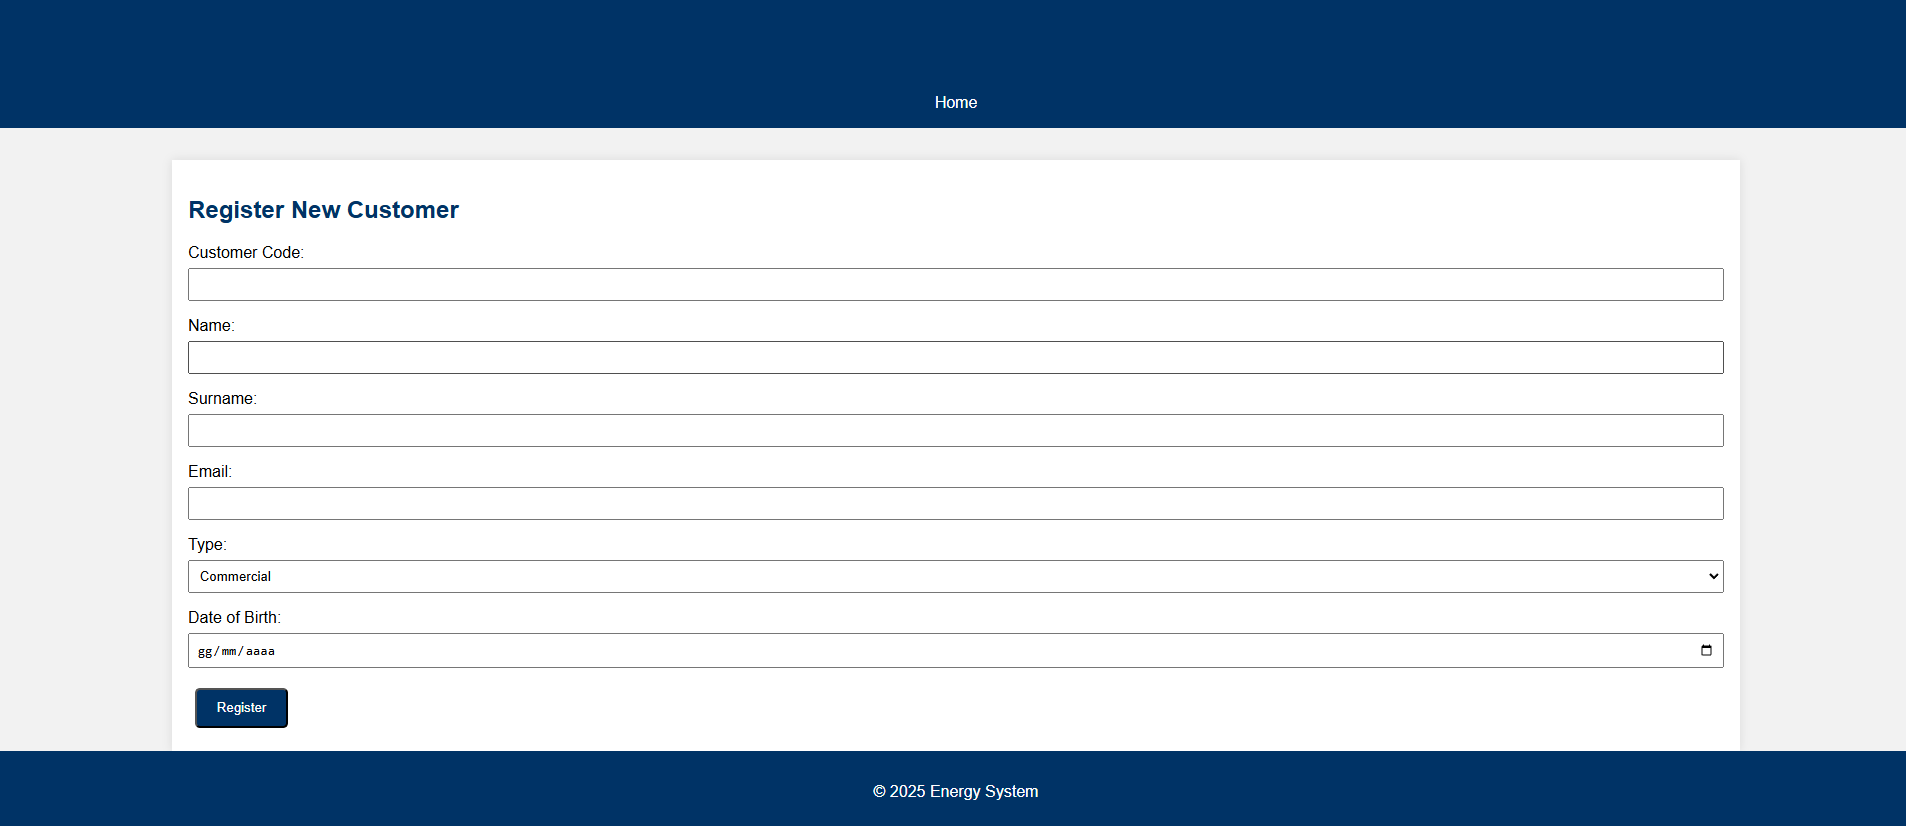
\includegraphics[width=\textwidth]{images/Op1.png}
    \caption{Register a new customer}
\end{figure}


\begin{figure}[H]
    \centering
    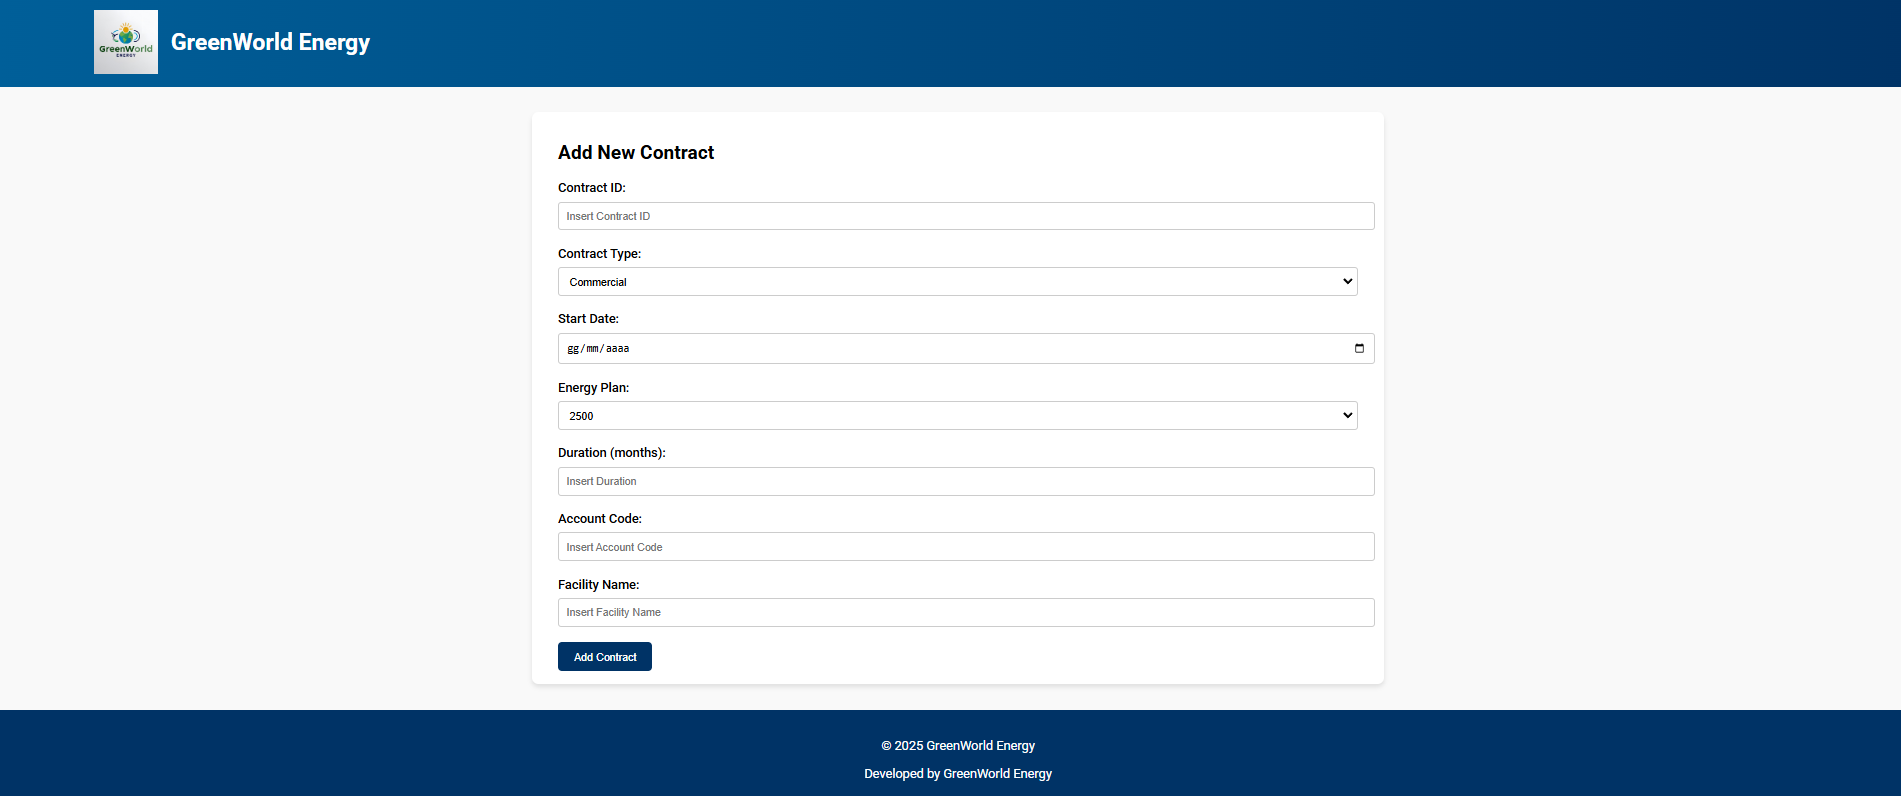
\includegraphics[width=\textwidth]{images/Op2.png}
    \caption{Add a new energy contract}
\end{figure}


\begin{figure}[H]
    \centering
    
\includegraphics[width=\textwidth]{images/Op3.png}
    \caption{Assign a facility to a management team}
\end{figure}


\begin{figure}[H]
    \centering
    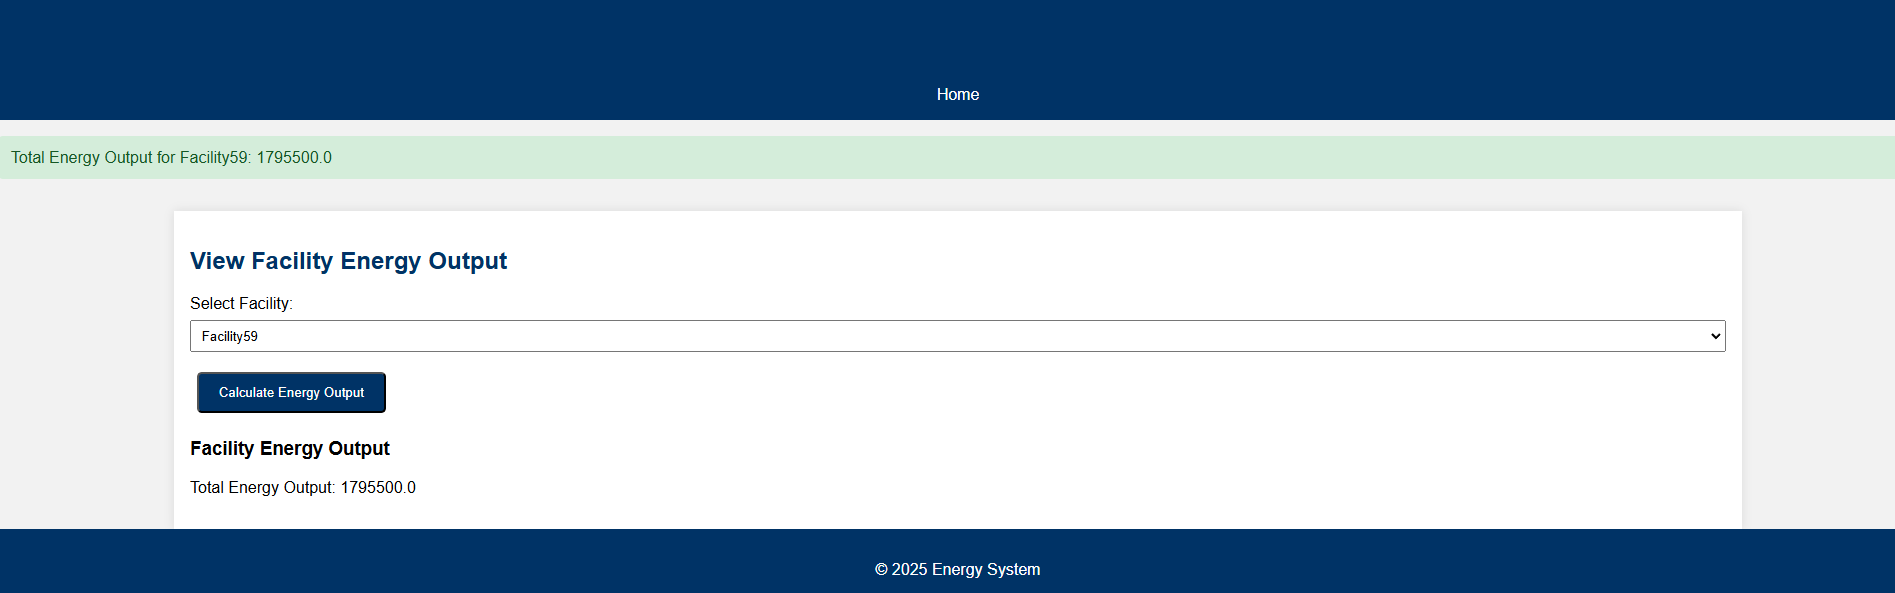
\includegraphics[width=\textwidth]{images/Op4.png}
    \caption{View the total energy output of a facility managed by the eldest employee}
\end{figure}


\begin{figure}[H]
    \centering
    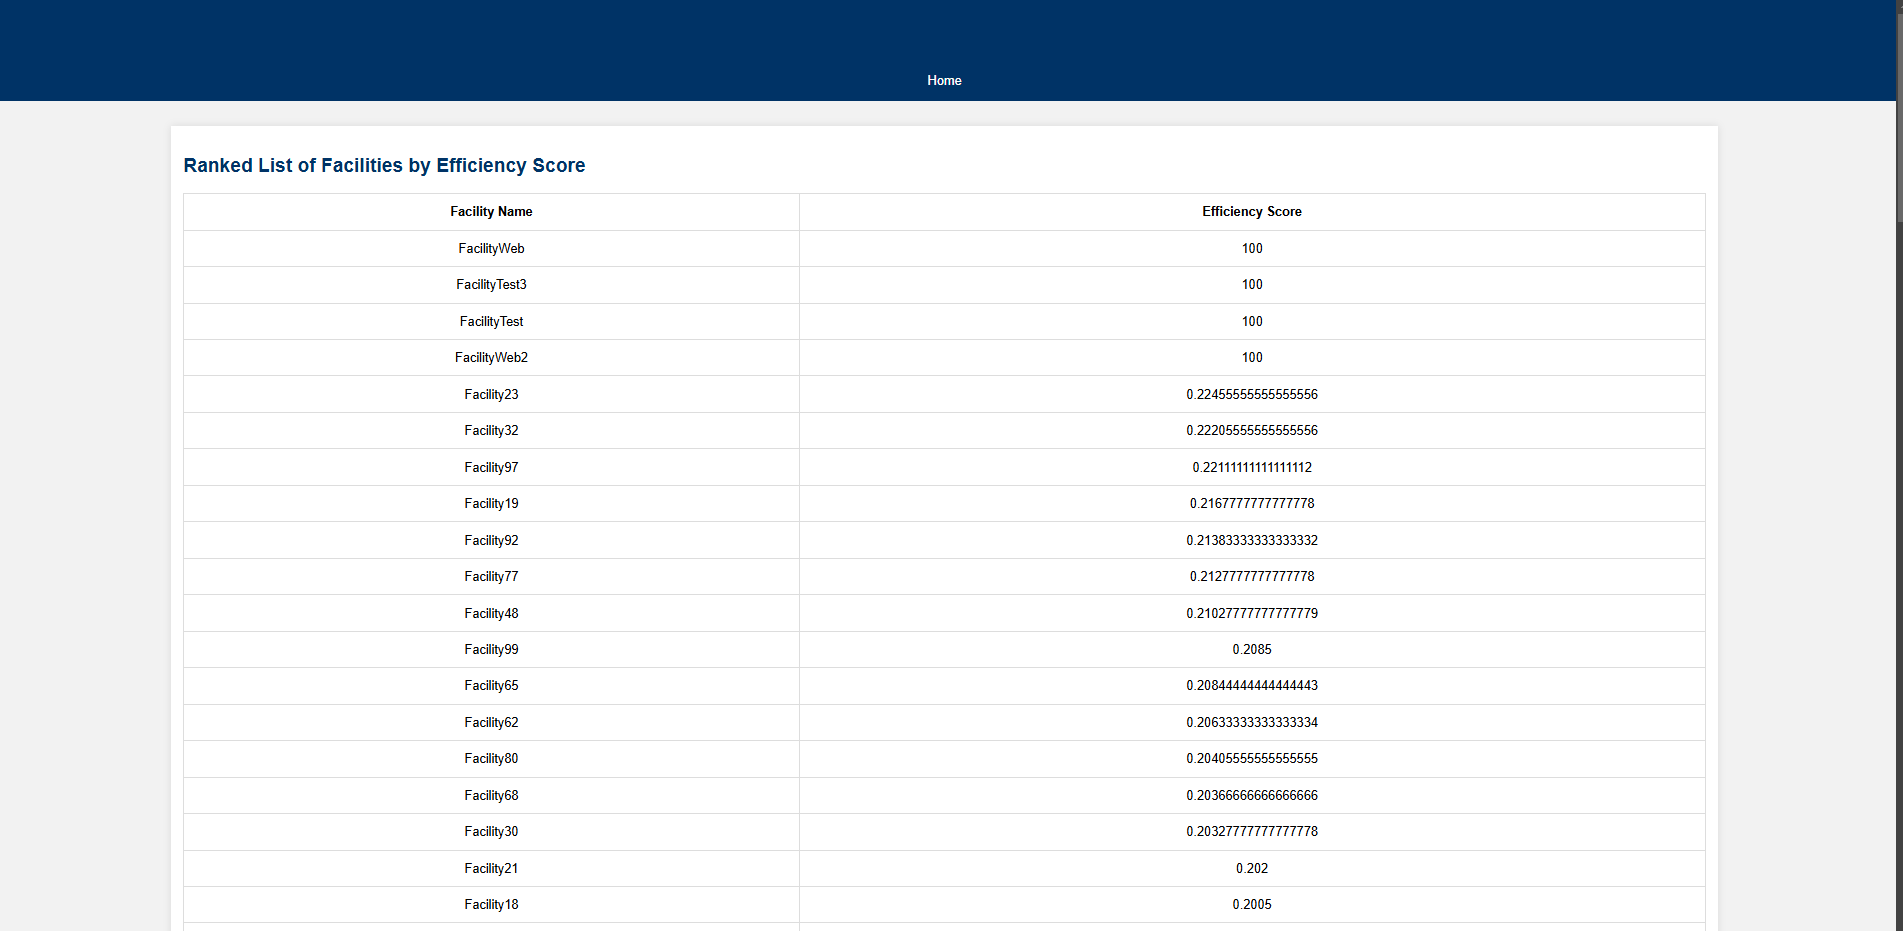
\includegraphics[width=\textwidth]{images/Op5.png}
    \caption{Print a ranked list of facilities based on their efficiency scores}
\end{figure}
\end{document}